\documentclass[11pt, oneside]{article}   	% use "amsart" instead of "article" for AMSLaTeX format
\usepackage{geometry}                		% See geometry.pdf to learn the layout options. There are lots.
\usepackage{textcomp}
\usepackage[colorlinks=true,urlcolor=blue, linkcolor=blue]{hyperref} 
\geometry{letterpaper}                   		% ... or a4paper or a5paper or ... 
\usepackage[parfill]{parskip}    		% Activate to begin paragraphs with an empty line rather than an indent
\usepackage{graphicx}				% Use pdf, png, jpg, or eps§ with pdflatex; use eps in DVI mode
								% TeX will automatically convert eps --> pdf in pdflatex		
\usepackage{amssymb}
\usepackage{amsmath}
\usepackage{relsize}

\usepackage{tikz}
\usetikzlibrary{arrows,automata}
\usetikzlibrary{positioning}


\tikzset{
    state/.style={
           rectangle,
           rounded corners,
           draw=black, very thick,
           minimum height=2em,
           text centered,
           },
}

\title{CS181 / CSCI E-181 Spring 2014 Final Project}
\author{
  David Wihl\\
  \texttt{davidwihl@gmail.com}
  \and
  Zachary Hendlin\\
  \texttt{zgh@mit.edu} 
}
%\date{}							% Activate to display a given date or no date


\begin{document}
\maketitle

\begingroup
\hypersetup{linkcolor=blue}
\tableofcontents
\endgroup

\section{Introduction}
Creating an agent to play Pacman required us considering a number of steps:
(1) Determining the latent class that each ghost belongs to based on its features (classification)
(2) Analyzing / visualizing the juciness of ghost by class (simple data analysis)
(3) Classification of capsule class (e.g. placebo or immunity to eating bad ghosts)
(4) A decision rule for the Pacman, either 'harded coded' or 'learned' (e.g. q-learning, policy interation, hidden markov models)

\section{Classification of Ghosts}
To gather sufficient data, we allowed the SampleAgent (provided intially in the code) to play until ~30 megabytes of ghost training data was captured on, to get data on feature vectors and associated 'juciness' point values of each.

We sought to classify ghosts as \{0, 1, 2, 3, 5\}, where all ghosts in category 5 are dangerous (e.g. induce a reward of -1000 points unless a helpful capsule is consumed first). Because of the huge payoff in eating a helpful capsule and then eating a 'bad' ghost, this is extremeley important.

We explored two methods for classifying the ghosts on the basis of their features.

First, we explored linear support vector machines (SVMs) using SK-Learn's Stochastic Gradient Descent classifier.

For classifying the category 5 ghosts, this approach was accurate 90.62 percent of the time. Our analysis found that while differences in the rewards associated with eating ghosts not from class 5 did differ by class, the most important thing for us to measure our performance on is the correct classification of dangerous (class 5 ghosts). See figure~\ref{fig:ghosts}.

\begin{figure}[h!]
  \centering
  \scalebox{0.7}{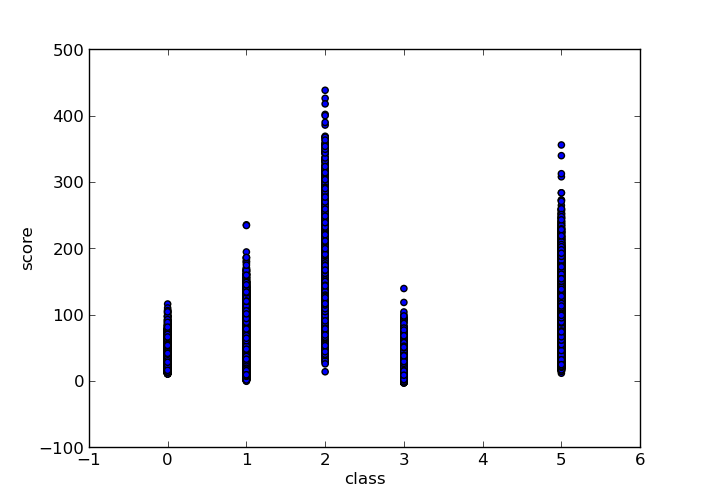
\includegraphics{scorebyclass}}
  \caption{Ghost Score by Class}
  \label{fig:ghosts}
 \end{figure}


We also used logistic regression classification, and achieved somewhat better results, with correct classification of class 5 ghosts 93.25 percent of the time.

We elected to use the logistic regression classification results to predict which class each ghost is in during runtime.

One additional way to tell if a ghost is category 5 (and hence dangerous) is it's change in distances from the Pacman. 'Bad ghosts' generally move closer and closer to the Pacman, whereas good ghosts do not demonstrate this behavior.

\section{Estimating the Juciness of Ghosts}

We had first thought about trying to pursue the highest point value ghosts and then follow them. But it turned out that the behavior of the aggressive 'bad ghost' dominated trying to eat regular ghosts.

As such, the data bore out that eating protective capsules and then pursuing the bad ghost was the most important thing for our Pacman to go pursue.

\section{Classification of Capsules and Placebos}
We wanted to determine which of the pills are helpful capsules and which are placebos. To do this, we first plotted the helpful capsules which we collected using the `-d' data collection function.

Here we determined that capsule feature values were very much clustered into three distinct clusters as shown in figure~\ref{fig:capsules}.
\begin{figure}[h!]
  \centering
  \scalebox{0.7}{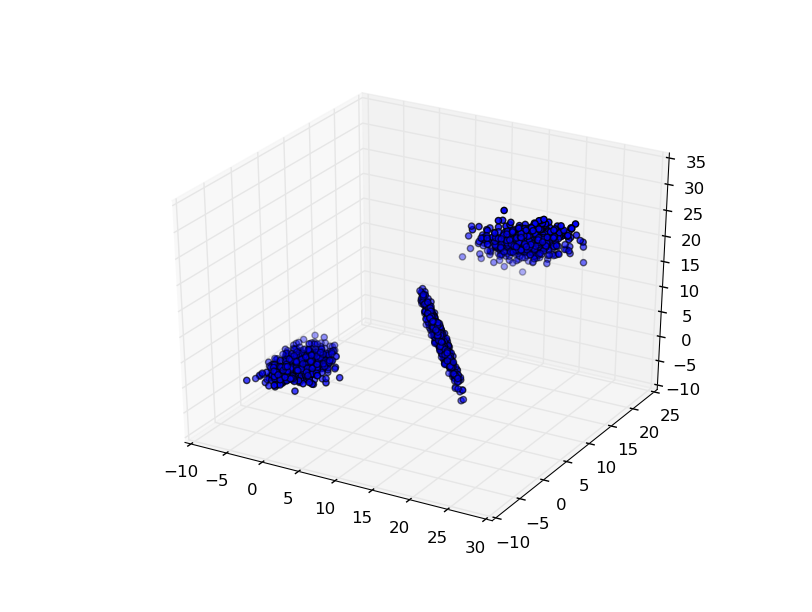
\includegraphics{good_capsule_plot}}
  \caption{Good Capsule Clusters}
  \label{fig:capsules}
 \end{figure}


This suggested that we could either fit Gaussians to these points as part of a generative approach, or apply something like K-means to find the clusters. Because the data were in three dimensions, we opted to use k-means for clustering, and initiated the model with kmeans++.

Because the three clusters were all positively identified, simply assigning a new value at run-time (for a capsule which may be a `good' or `placebo'), we instead used the `score' attribute to evaluate the distance from the centroid the data point would have been assigned to. We are agnostic to which centroid the capsule would be assigned to but we are very sensitive to the score assigned (e.g. the distance from the centroid assignment), with larger distances being worse.

From our positive training data, we found values of $0$ to $-118$ as the `good' range of objective function values. Any value $<-118$ would likely be a placebo capsule.

So at runtime we score each capsule based on its $3\times1$ feature vector and we consider the `best' capsule the one with the maximum objective function value when scored.

\section{Decision Rules}

\subsection{Reinforcement Learning}
We first attempted to implement a Q-learning based approach\cite{sutton}, but very quickly found this to be infeasible due to the extremely large state space.

For a 20x20 matrix five ghosts (each with a class of 1 to 5), five capsules (each with a 1/0 classification), and our Pacman's ability to make four moves, our (state, action) space is $(20^2)^{5^5} \times (20^2)^{5^2} \times (20^2) \times 4$.

It is clear that we get to such a large state space that we can't reasonably visit every single state. We tried to reduce the state space by only keeping track of the 'good' capsules and the 'bad' ghosts but we still found this state space to be too large to fit. 

Although we coded up Q-learning, ran it for a while, and tried to reduce the dimensionality of the state space, we still found this state space to be too large.

\subsection{Rules Engine}
Our next approach was to build a procedural rules engine inspired by a Markov process. In other words, the rules engine did not require any historical data and would simply decide the next action based on the current state of the game.

The other reason for building a rules engine was to better grapple with the game dynamics to see if the model could be significantly simplified. We believe we were successful as the game came down to a straightforward finite state machine. 

We iterated through more than 10 different heuristics. Taken over 10 different seeds, our average score over 50 games of 200 moves went from a dismal $-7390$ to a reasonable $933$.

\subsection{Finite State Machine}

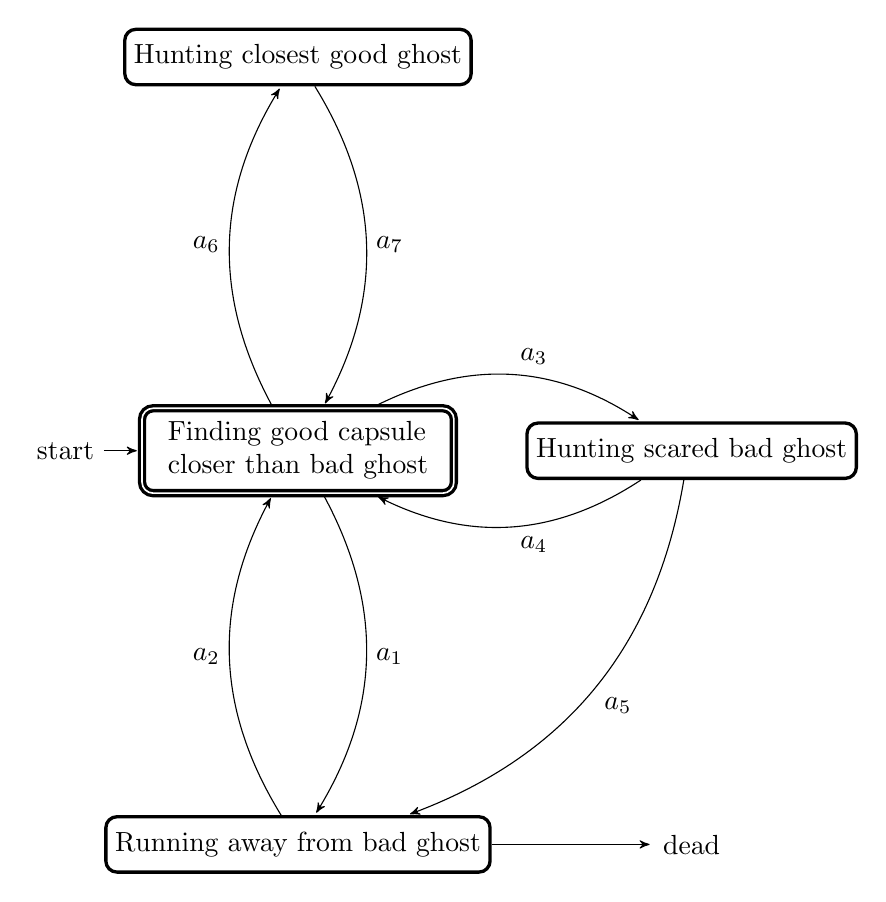
\begin{tikzpicture}[>=stealth',shorten >=1pt,auto,node distance=5cm]
 	\tikzstyle{every state}=[align=center]

	\node[initial,state,accepting] (S1)      
			{
				\begin{tabular}{l}
				Finding good capsule\\
				closer than bad ghost
				\end{tabular}
			};
	\node[state]         (S2) [below of=S1]  {Running away from bad ghost};
	\node[state]         (S3) [right of=S1] {Hunting scared bad ghost};
	\node[state]	   (S4) [above of=S1] {Hunting closest good ghost};
	\node[state,draw=none,fill=none]	   (die) [right of=S2] {dead};
	
	\path[->] (S1) edge  [bend left]           node  {$a_3$} (S3);
	\path[->] (S3) edge  [bend left]           node {$a_4$} (S1);
	
	\path[->] (S1) edge  [bend left]           node [align=right] {$a_1$} (S2);
	\path[->] (S2) edge  [bend left]           node {$a_2$} (S1);
	
	\path[->] (S3) edge [bend left]          node {$a_5$} (S2);
	
	\path[->] (S1) edge  [bend left]           node {$a_6$} (S4);
	\path[->] (S4) edge  [bend left]           node {$a_7$} (S1);

	\path[->] (S2) edge node {} (die);
	
\end{tikzpicture}

where:
\begin{description}
	\item[$a_1$] bad ghost closer than good capsule
	\item[$a_2$] good capsule closer than bad ghost
	\item[$a_3$] bad ghost is scared and within range
	\item[$a_4$]bad ghost is out of range
	\item[$a_5$]bad ghost will no longer be scared soon
	\item[$a_6$]no good capsule in range
	\item[$a_7$]good capsule now in range
\end{description}


The Rules Engine provided the following advantages:
\begin{description}
	\item[Understanding Game Dynamics]We had a much better grasp of the \emph{keys to success} to the game.
	\item[Key Factors]We could distill key factors that would be difficult if not impossible to discover by exploration, such as the equivalence between clock ticks and Manhattan distance between objects.
	\item[Latent Factors]One of the key pieces of information was the time remaining before scared bad ghost reverted to normal. We found this by careful examination of the game code. It would have been difficult if not impossible to discover this feature by exploration.
	\item[No history]With our ghost and capsule classifiers, we could immediately evaluate the best option from the current board.
	\item[Flexibility]Since only the current state is necessary our rules engine would be flexible enough to handle more dynamics than in the current game. \bf{The entire board could resize,  walls could move, capsules could be in motion and the bad ghost could change between time clicks and the Rules Engine would still find  a reasonably good action.}
\end{description}



\subsection{Parameter Tuning}
We defined two configuration settings:
\begin{description}
	\item[Capsule Threshold]As mentioned in the Classification of Capsules, we determined a capsule score. We had to evaluate whether it was worth risking targeting a capsule that might turn out to be a placebo. Interestingly, if we played too conservative and tried to reach only certainly good capsules, our average score decreased. It paid to aggressively chase capsules even with a lower certainty. See figure~\ref{fig:threshold}.
	\item[Time Buffer]We knew how many ticks before a scared ghost reverted to a bad ghost, but did not know where precisely the scared ghost would move. So we had to determine the appropriate margin to give the scared bad ghost lest it turn on us. See figure~\ref{fig:buffer}.
\end{description}
While both of these parameters could have been found via regression, it would have required extensive modifications to the provided game execution code to get the appropriate harness in place. We simply opted to manually iterate on these parameters. This involved 21 tuning runs (200 moves, 50 games, 20 different seeds) for over 4M moves used for tuning.
\begin{figure}[h!]
  \centering
  \scalebox{0.7}{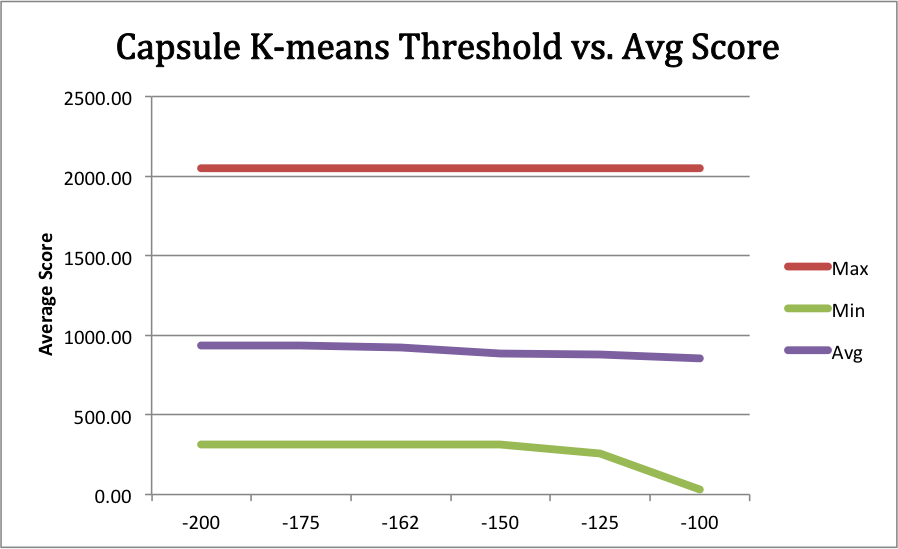
\includegraphics{threshold_tune}}
  \caption{Capsule Threshold Tuning}
  \label{fig:threshold}
 \end{figure}

\begin{figure}[h!]
  \centering
  \scalebox{0.7}{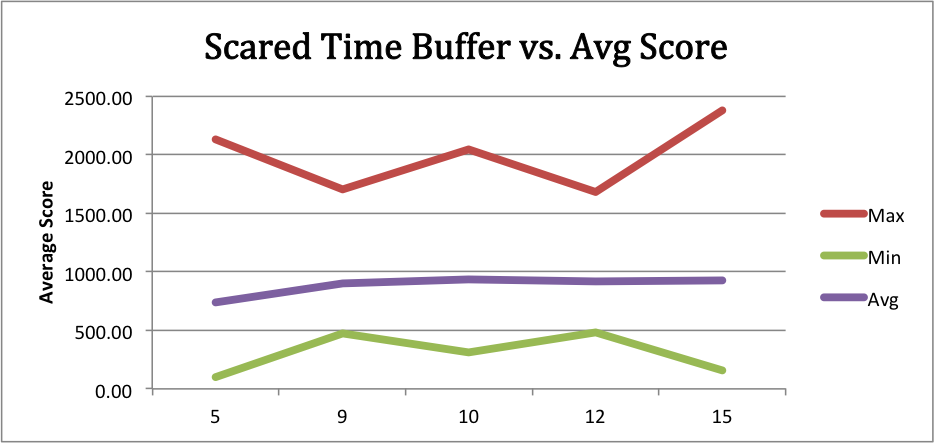
\includegraphics{buffer_tune}}
  \caption{Time Buffer Tuning}
  \label{fig:buffer}
 \end{figure}


\subsection{Scores Across Different Seeds}

To ensure the reliability of the Rules Engine, we tested against 20 different seed values $s = \{1..20\}$. While the min and max scores for a given seed could vary significantly, the overall average across multiple seeds was quite consistent once we tuned the parameters. Interestingly, the Capsule Threshold improved the minimum score, while the Time Buffer increased the maximum score. See figure~\ref{fig:seeds}. Across all seeds we tested, the average score was always positive, giving us confidence in the flexibility of the Rules Engine. To visualize distribution of losing vs winning scores, see figure~\ref{fig:3dscore}.

\begin{figure}[h!]
  \centering
  \scalebox{0.7}{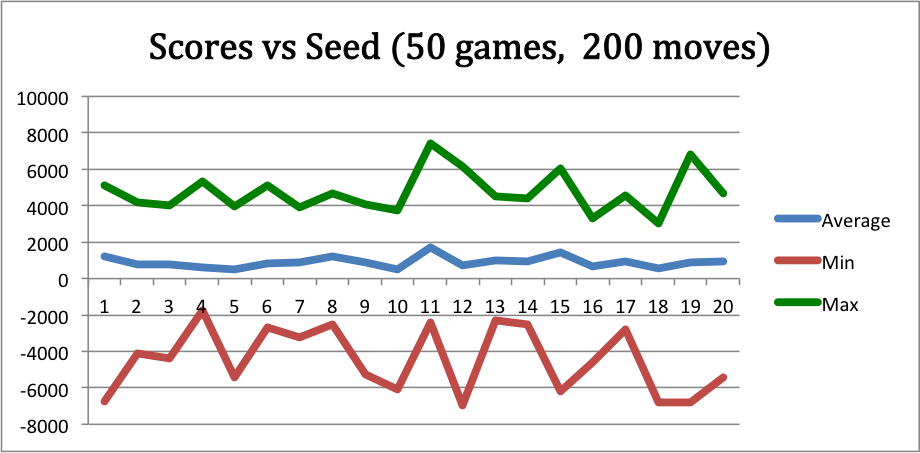
\includegraphics{scoresVseed}}
  \caption{Scores Across 20 Different Seeds, Tuned Parameters}
  \label{fig:seeds}
 \end{figure}

\begin{figure}[h!]
  \centering
  \scalebox{0.7}{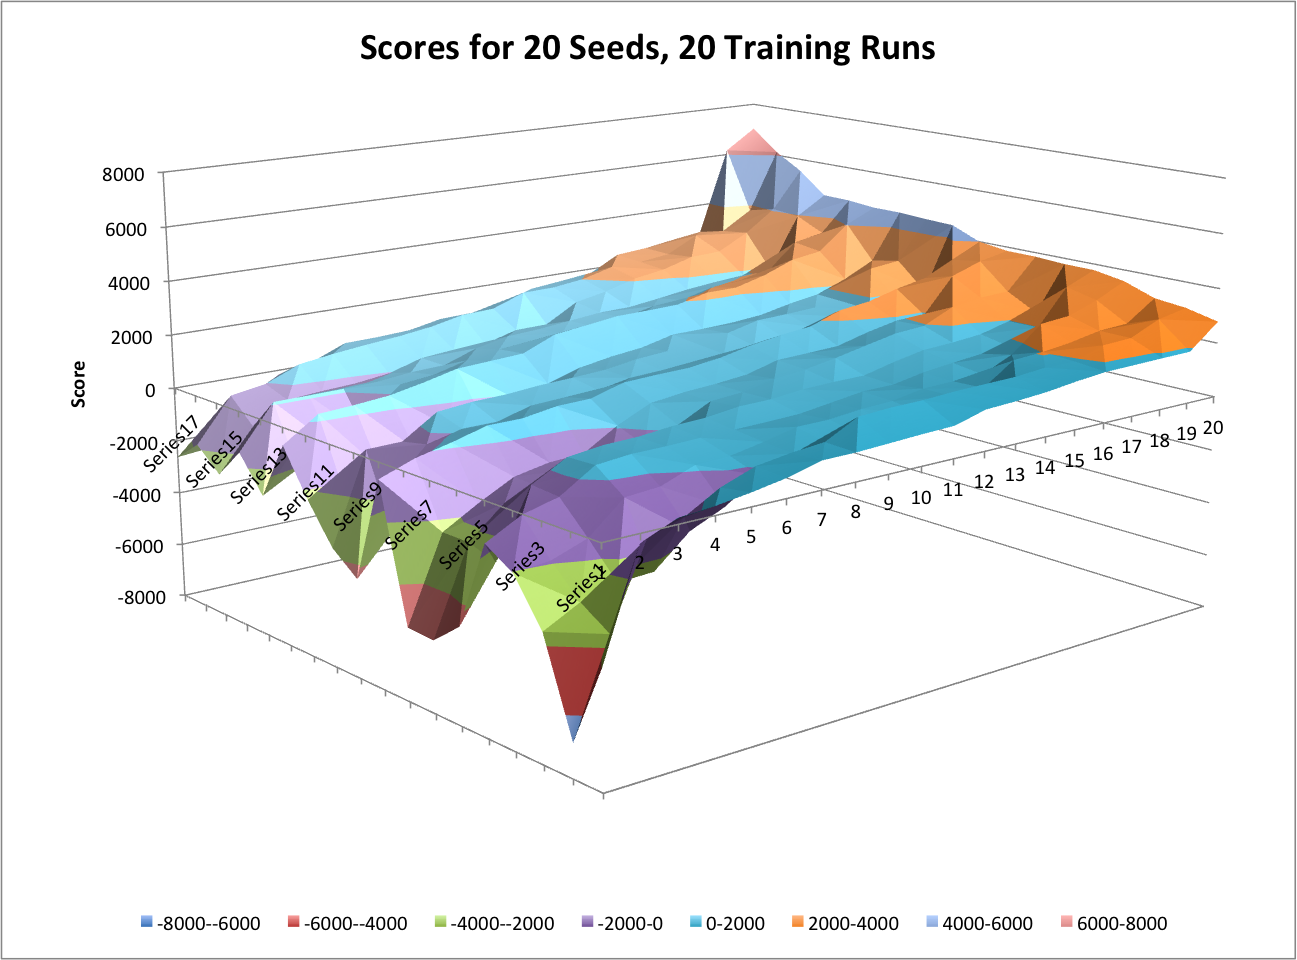
\includegraphics{3dscore}}
  \caption{Winning more than losing}
  \label{fig:3dscore}
 \end{figure}

\section{Other Methods Considered}

Not satisfied with our Rules Engine, we continued to evaluate and experiment with other Machine Learning techniques to find a potentially better solution.

\subsection{Expectimax}

Given the simplified state machine, Expectimax would not have yielded an improvement. The game dynamics were so highly contingent upon the eating or being eaten by the bad ghost that doing a deep tree of probabilities would not have been beneficial especially when we found the deterministic relationship between Manhattan distance and clock ticks before the scared ghost would revert.

\subsection{Alpha-Beta Search}

An older, commonly used game playing strategy is Alpha-Beta Pruning.\cite{russell} Had we needed to look further into the future, this technique would have likely been significantly more efficient than Expectimax. We could have built a value tree and pruned off the courses of action that did not yield valuable results. Once again, given our simplified model, pursuing even this rather simple implementation became unnecessary.

\subsection{Hidden Markov Model}
The main challenge to implementing a HMM for this problem was that the state transitions were not in the form of an acyclic digraph. It would be possible to model sequential transitions using the observed data but given the dimensionality, we were not confidential a good result would emerge in a reasonable time.

One other complication was finding a suitable HMM library given the cluster execution environment. (For example, we could not use \href{www.ghmm.org}{GHMM} due to a C library dependency.) Ultimately, we did find Roland Memisevic's \href{http://www.iro.umontreal.ca/~memisevr/code/hmm.py}{implementation} and did some initial experimentation.

\subsection{Probabilistic Graphical Model}

The most interesting potential Machine Learning technique given the Finite State Machine would be a Probabilistic Graph Model.\cite{koller} A PGM would likely circumvent the acyclic digraph limitations of HMM. It would not replace the rules engine in cases where the scared ghost was within range. However, it may have discovered a better escape strategy by modeling the bad ghost's behavior. It also may have discovered a better means of hunting good ghosts and trading off capsule score vs distance. Unfortunately, we did not have time to implement this in a quality form. We were not able to find any readily available ``off-the-shelf" libraries that would have help our implementation. This is a further area of research for us.

\section{Conclusion}
A combination of Machine Learning and traditional techniques is more powerful than using one set of techniques alone. This exercise was a useful reminder of \href{http://en.wikipedia.org/wiki/Law_of_the_instrument}{Maslow's Hammer} that  ``if all you have is a hammer, everything looks like a nail." Machine Learning provides a valuable set of additional tools to add to the proverbial utility belt. The most effective solution in this case was a combination of human derived rules coupled with Machine Learning techniques. 

Thank you for a stimulating and instructive class.

\begin{thebibliography}{1}

 \bibitem{sutton}\emph{Reinforcement Learning}, Sutton \& Barto, 1998, ISBN-10: 0-262-19398-1
 
 \bibitem{russell}\emph{Artificial Intelligence: A Modern Approach}, Russell and Norvig, Third Edition, 2010, ISBN 978-0-13-604259-4, pg 167
 
 \bibitem{koller}\emph{Probabilistic Graphical Models}, Koller and Friedman, 2009, ISBN 978-0-262-1319-2
 
  \end{thebibliography}

\end{document}  
